% Supplementary material of the paper. The figures and the tables are the files that the
% analysis scripts write to app/nlp/evaluation/results/video-v2/ (see the README,
% "Numbers, tables and figures"); nothing here is typed by hand. Rebuild with
%   cd supplementary && latexmk -pdf supplementary.tex
\documentclass[11pt]{article}
\usepackage[a4paper,margin=2cm]{geometry}
\usepackage[T1]{fontenc}
\usepackage[utf8]{inputenc}
\usepackage{lmodern}
\usepackage{booktabs}
\usepackage{graphicx}
\usepackage{amsmath,amssymb}

\renewcommand{\thetable}{S\arabic{table}}
\renewcommand{\thefigure}{S\arabic{figure}}
% artigo/: outputs of gerar_figuras_artigo.py; latex/: outputs of the other scripts
\newcommand{\artigo}{../app/nlp/evaluation/results/video-v2/artigo}
\newcommand{\resultados}{../app/nlp/evaluation/results/video-v2/latex}
\graphicspath{{../app/nlp/evaluation/results/video-v2/artigo/}{../app/nlp/evaluation/results/video-v2/latex/figuras/}}

\title{Supplementary material\\[4pt]
\large Toxicity Detection in Brazilian Portuguese Video Transcripts: An Annotated Corpus, a
Three-Level Classifier and a Verbal-Toxicity Score for Children's Video Search}
\date{}

\input{\resultados/numeros}

\begin{document}
\maketitle

\noindent This file holds three tables and four figures that the paper cites but does not
print. They are generated, like every number in the paper, by the scripts of this
repository from the stored result files of the video-disjoint run with the revised labels.
Section titles below are those of the paper.

\begin{itemize}
  \item Table~\ref{tab:halving}: Stage 2 of the hyperparameter search (section
        ``Hyperparameter selection'').
  \item Figure~\ref{fig:f1-classe-comparativo}: per-class F1 of BERTimbau and of the two
        strongest fixed baselines (section ``Per-class analysis'').
  \item Figure~\ref{fig:calibracao}: reliability diagrams of the reference model (section
        ``Calibration and sensitivity of the score'').
  \item Figure~\ref{fig:score-por-classe}: verbal-toxicity score by annotated class (section
        ``Behaviour of the verbal-toxicity score'').
  \item Figure~\ref{fig:estratos}: verbal-toxicity score of each case-study video, by
        query (section ``Separation between strata'').
  \item Table~\ref{tab:limiares-estudo-caso}: case-study outcome at the a priori threshold
        and at every exploratory threshold (section ``Detection at the threshold fixed in
        advance'').
  \item Table~\ref{tab:simulacao-variantes}: sampling simulation under alternative video
        models (section ``What sampling sparsely costs'').
\end{itemize}

\input{\artigo/tab-halving}

\begin{figure}[!h]
\centering
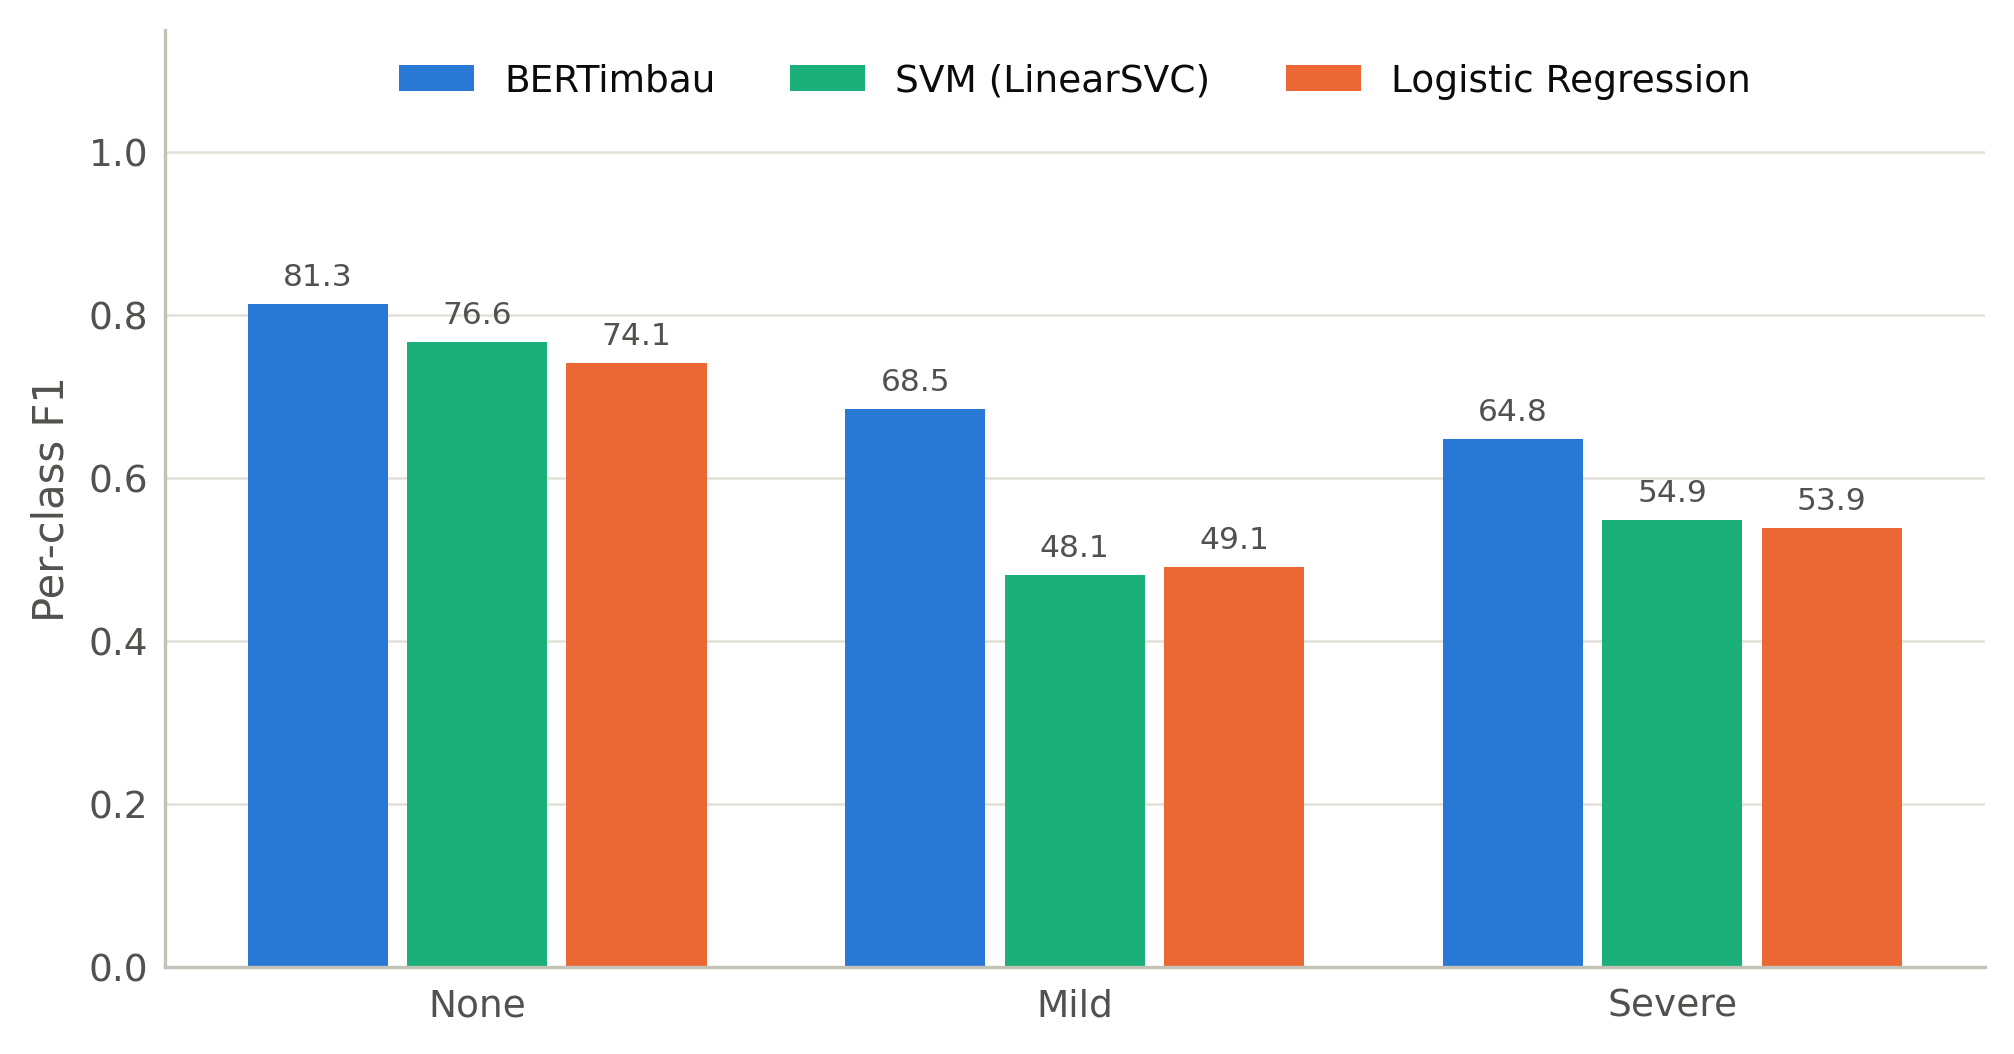
\includegraphics[width=0.6\textwidth]{fig06-f1-por-classe.png}
\caption{Per-class F1 on the held-out test set: BERTimbau vs.\ the two strongest fixed
baselines in cross-validation.}
\label{fig:f1-classe-comparativo}
\end{figure}

\clearpage
\begin{figure}[!h]
\centering
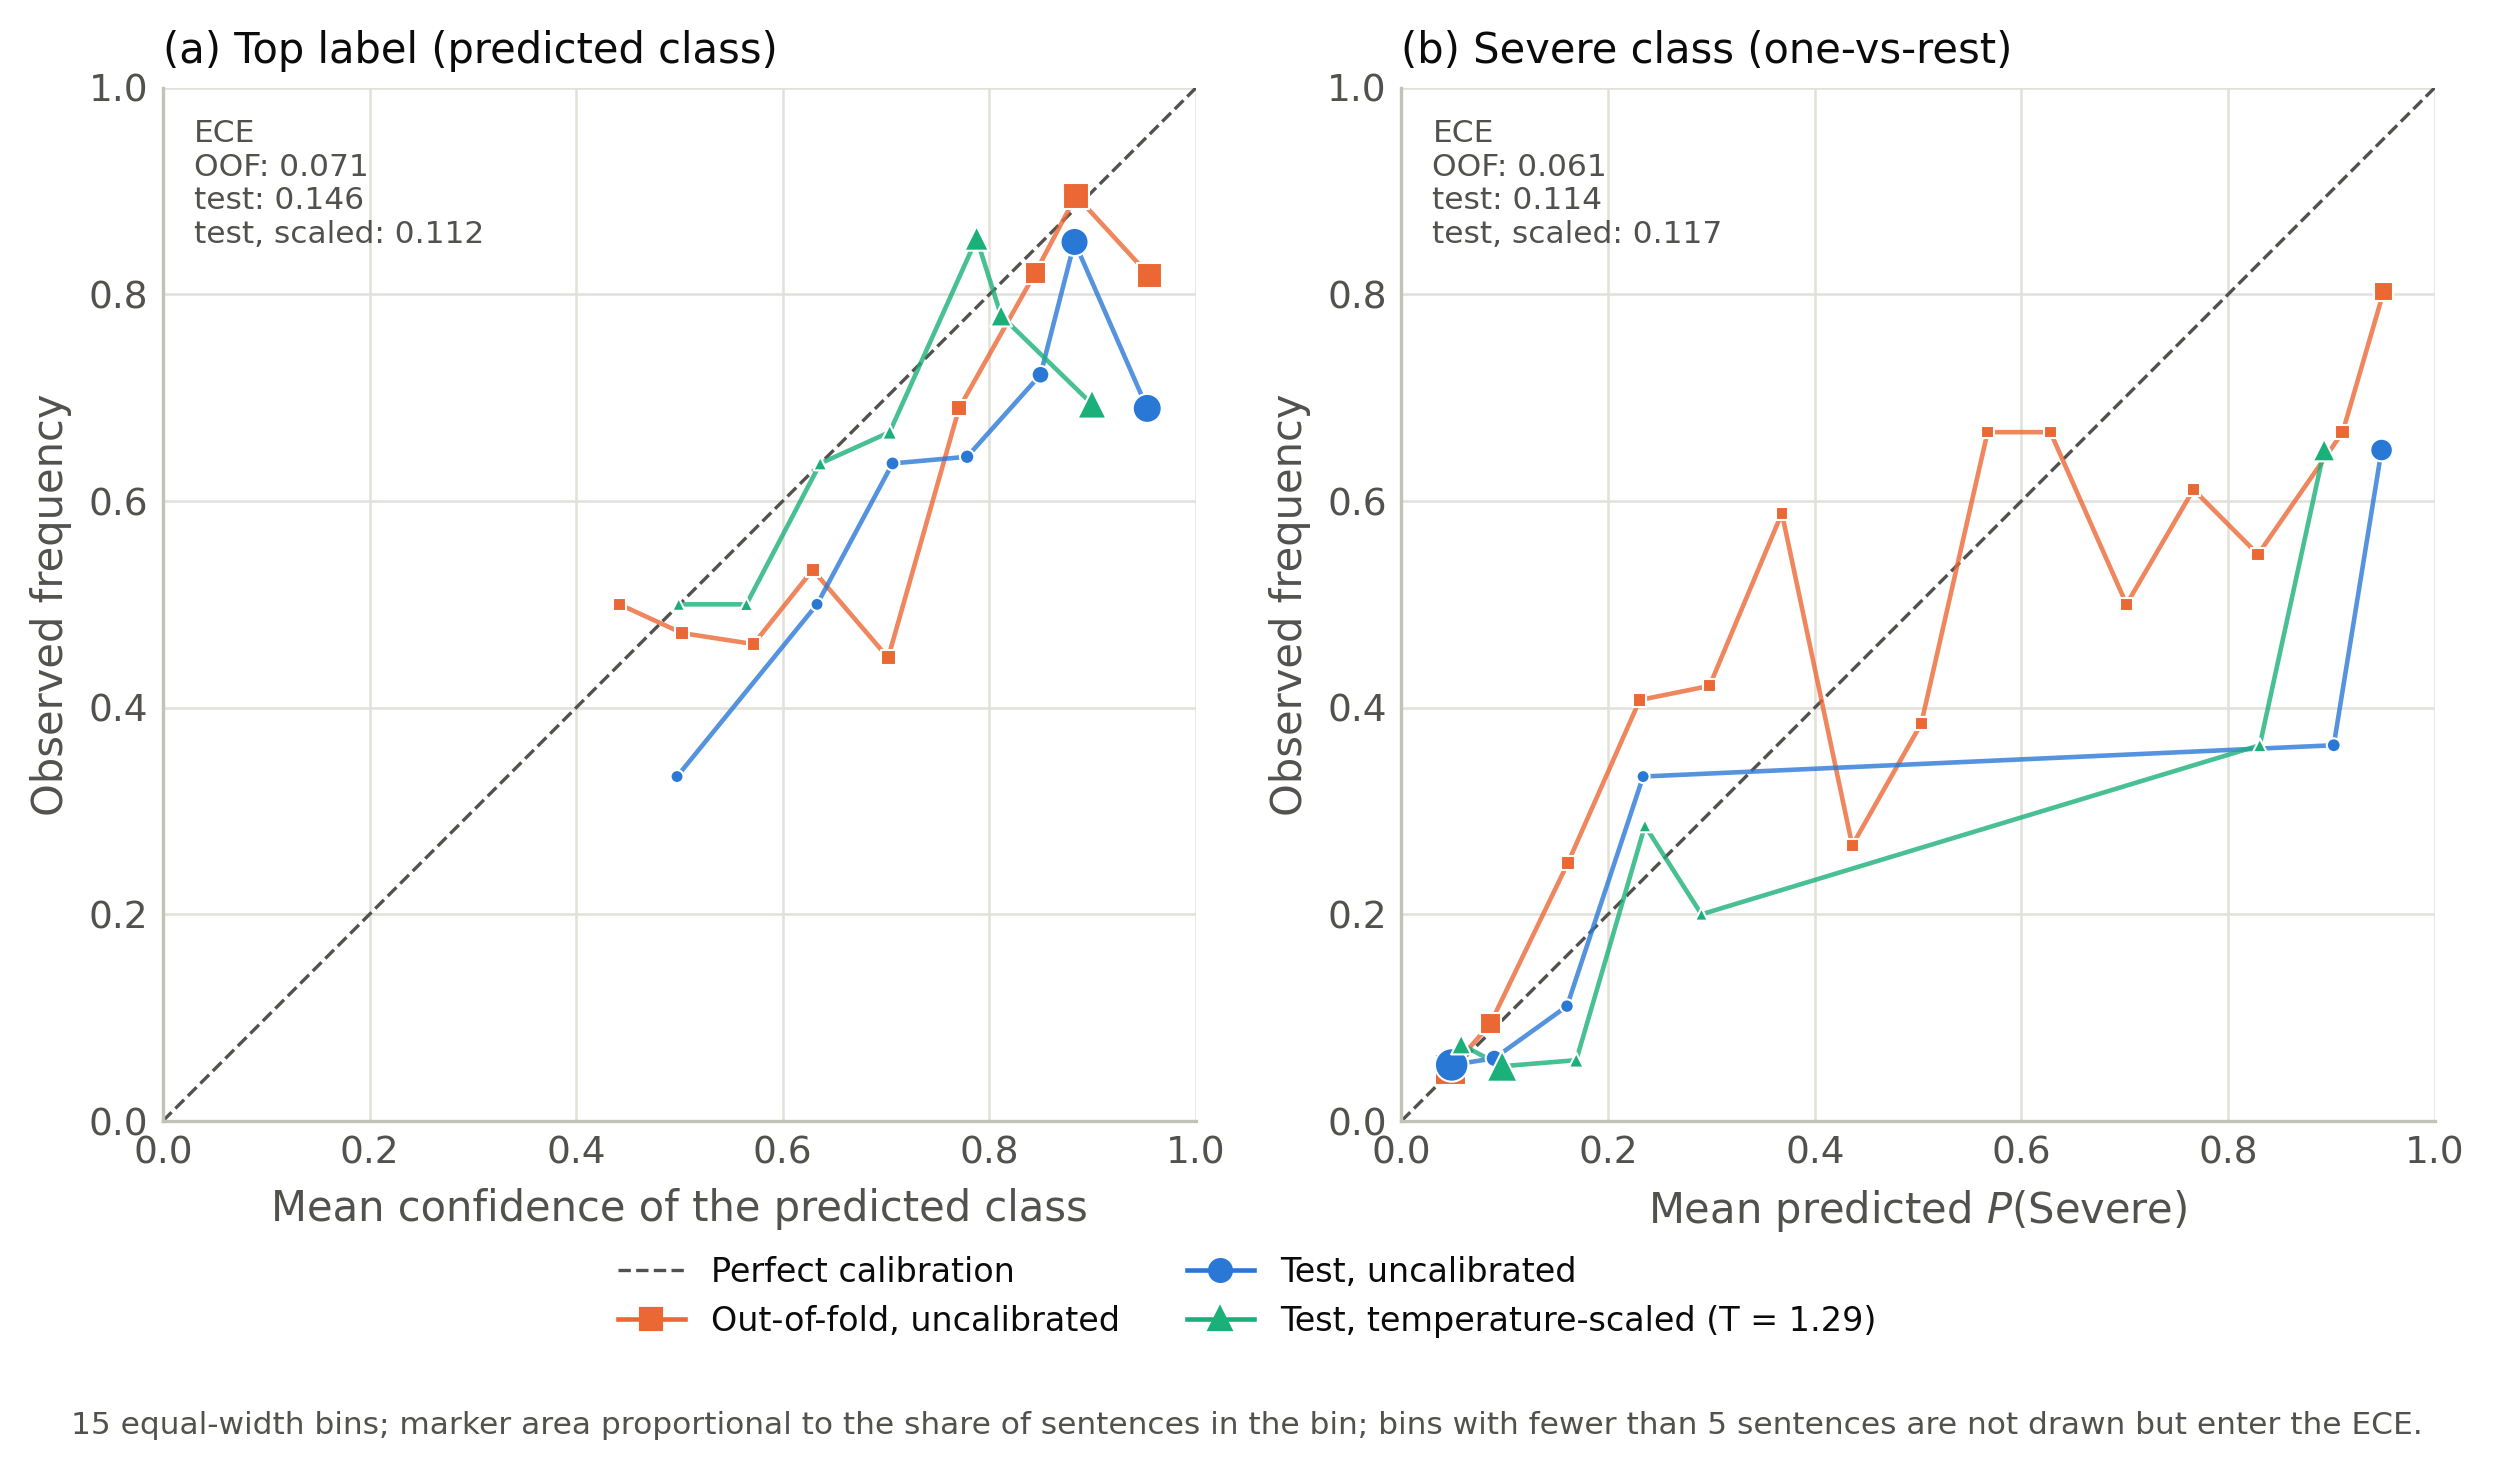
\includegraphics[width=\textwidth]{fig-calibracao.png}
\caption{Reliability diagrams of the reference model: (a) confidence of the predicted class
and (b) probability of the Severe class, one-vs-rest, out of fold on the training split and
on the held-out test set, before and after temperature scaling fitted out of fold.}
\label{fig:calibracao}
\end{figure}

\begin{figure}[!h]
\centering
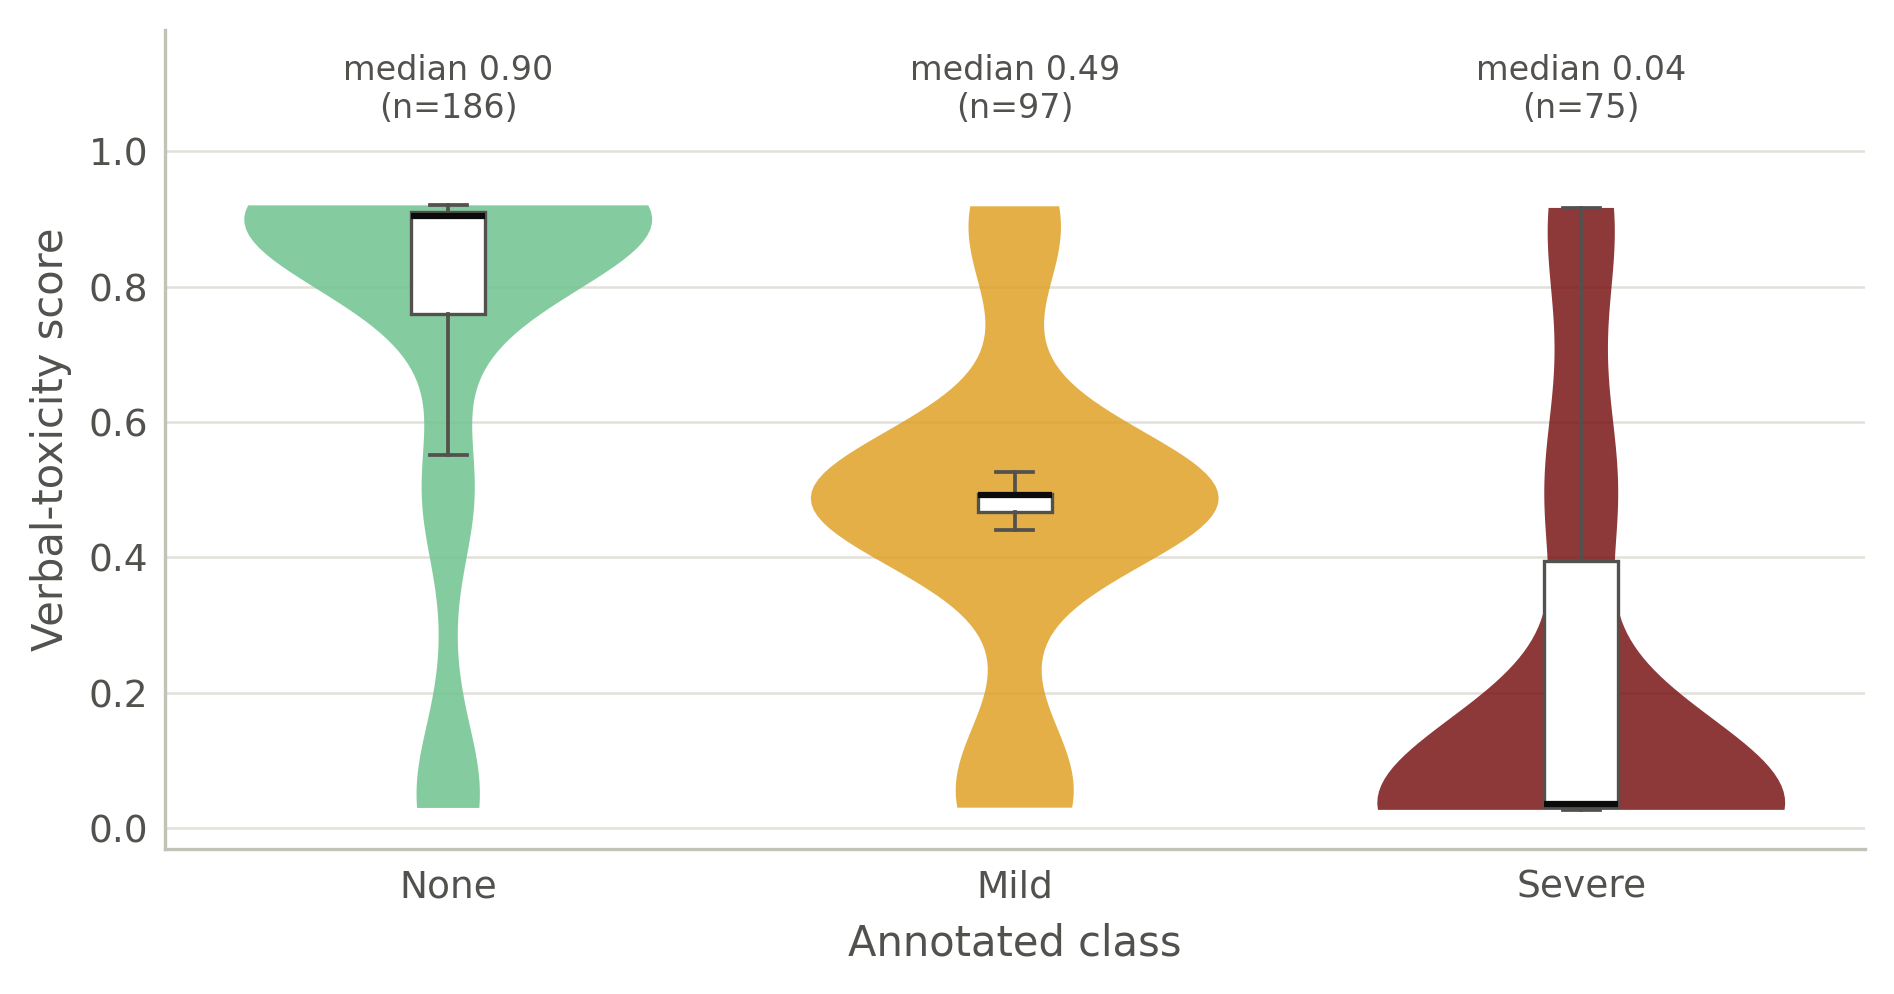
\includegraphics[width=0.6\textwidth]{fig10-score-por-classe.png}
\caption{Distribution of the verbal-toxicity score by annotated class, on the held-out test
set (reference model).}
\label{fig:score-por-classe}
\end{figure}

\begin{figure}[!h]
\centering
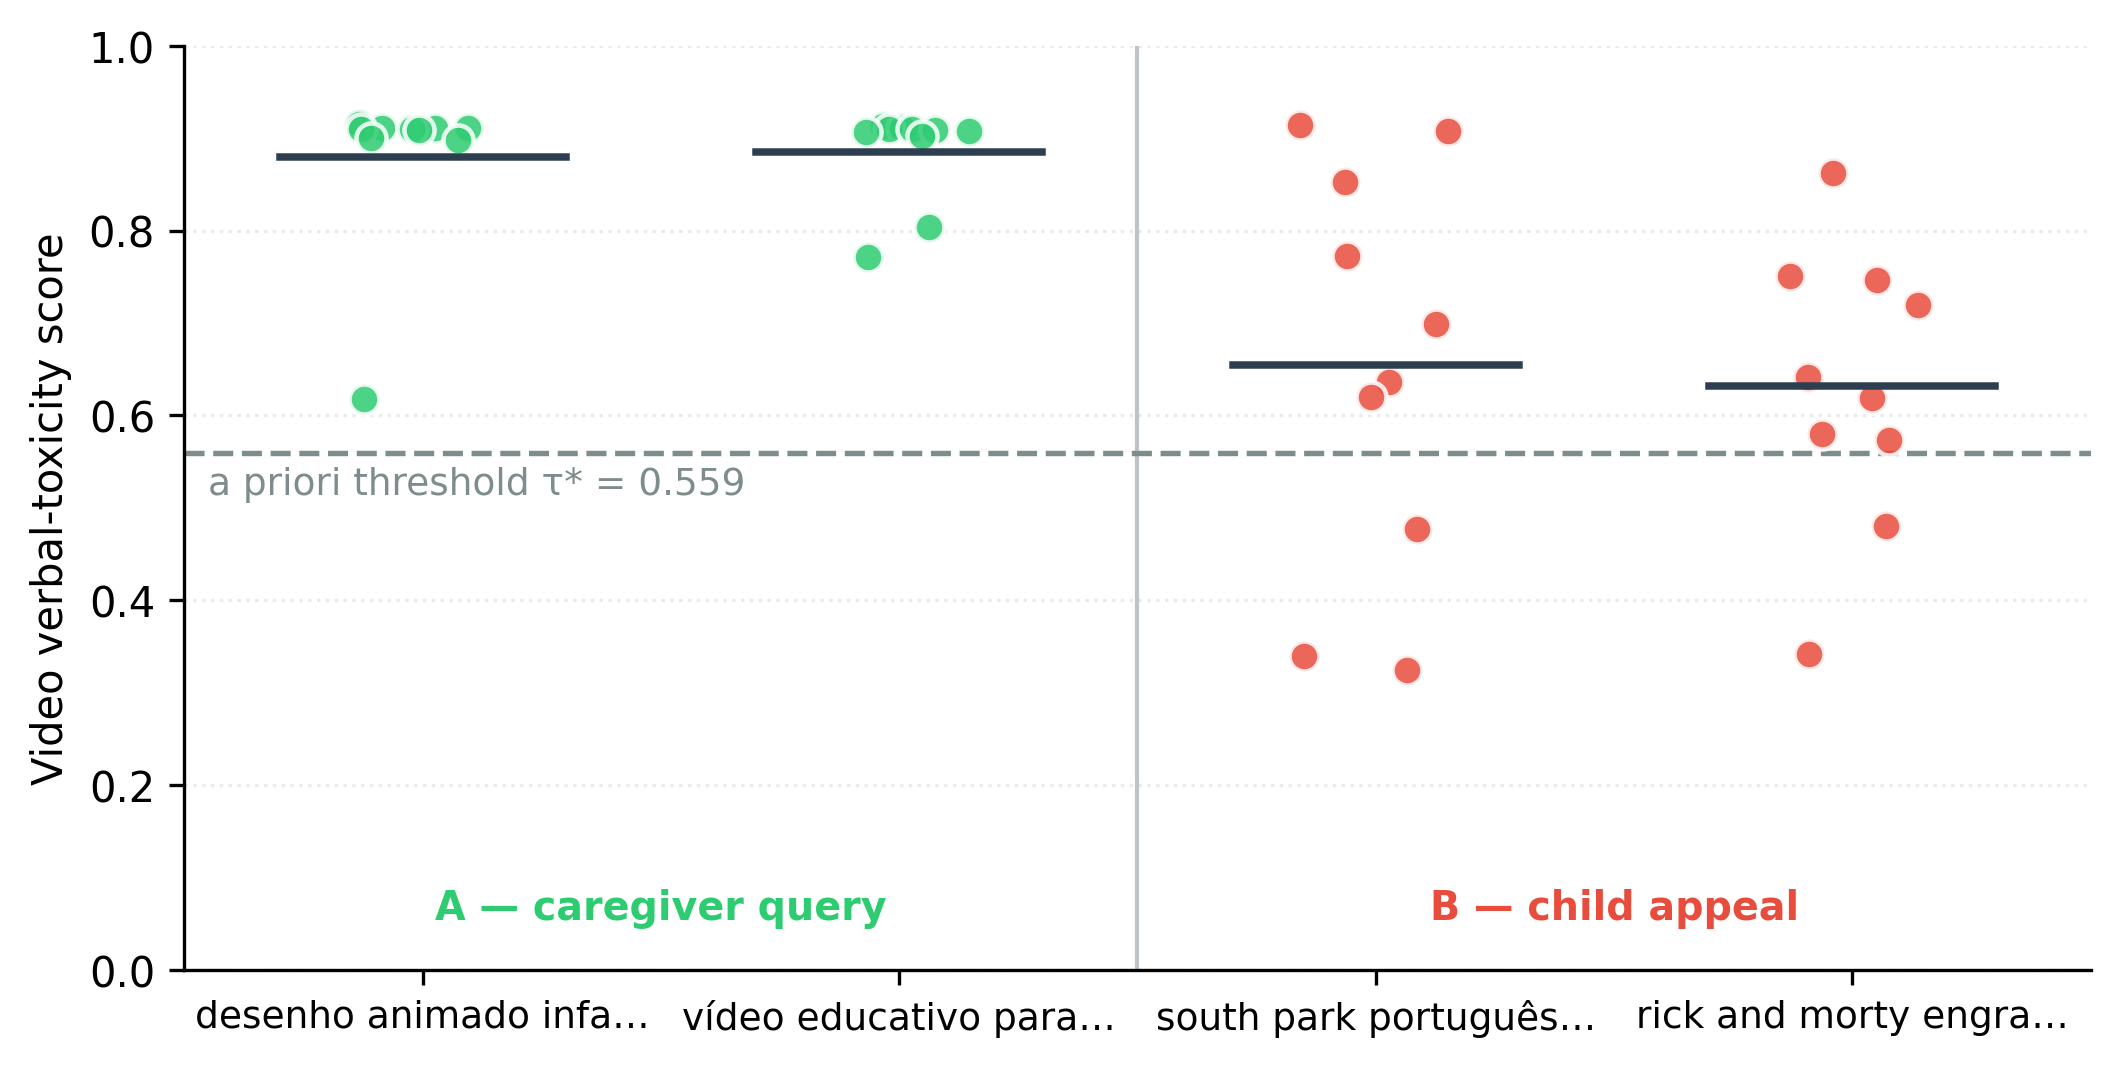
\includegraphics[width=\textwidth]{fig11-estratos.png}
\caption{Verbal-toxicity score (toxicity filter only) of the \yskEstNVideos{} case-study
videos, one point per video; bars mark the mean of each query, and the line the a priori
threshold $\tau^{*}$. Query terms are given verbatim in Brazilian Portuguese, since they are
inputs to the service.}
\label{fig:estratos}
\end{figure}

\clearpage
\input{\resultados/tabelas/tab-limiares-estudo-caso}

\input{\resultados/tabelas/tab-simulacao-variantes}

\end{document}
